\documentclass[journal,10pt,twocolumn]{article}
\usepackage{graphicx}
\usepackage[none]{hyphenat}
\usepackage{graphicx}
\usepackage{listings}
\usepackage[english]{babel}
\usepackage{graphicx}
\usepackage{caption} 
\usepackage{hyperref}
\usepackage{booktabs}
\usepackage{array}
\usepackage{amsmath}   % for having text in math mode
\usepackage{extarrows} % for Row operations arrows
\usepackage{listings}
\lstset{
  frame=single,
  breaklines=true
}
  
%Following 2 lines were added to remove the blank page at the beginning
\usepackage{atbegshi}% http://ctan.org/pkg/atbegshi
\AtBeginDocument{\AtBeginShipoutNext{\AtBeginShipoutDiscard}}


%New macro definitions
\newcommand{\mydet}[1]{\ensuremath{\begin{vmatrix}#1\end{vmatrix}}}
\providecommand{\brak}[1]{\ensuremath{\left(#1\right)}}
\providecommand{\norm}[1]{\left\lVert#1\right\rVert}
\newcommand{\solution}{\noindent \textbf{Solution: }}
\newcommand{\myvec}[1]{\ensuremath{\begin{pmatrix}#1\end{pmatrix}}}
\let\vec\mathbf

\begin{document}

\begin{center}
\title{\textbf{Equation  of Line}}
\date{\vspace{-5ex}} %Not to print date automatically
\maketitle
\end{center}
\setcounter{page}{1}

\section{11$^{th}$ Maths - Chapter 10}
This is Problem-5 from Exercise 10.2
\begin{enumerate}
\item Instersecting the x-axis at a distance of 3 units to the left of origin with slope of -2.
\\

\solution 
\\
\begin{align}		
m=-2\\
\vec{m}=\myvec{1\\-2}
\end{align}
\begin{align}
\vec{A}=\myvec{-3\\0}
\end{align}
$\implies$ The normal vector $\vec{n}$ to the line is given as
\begin{align}
\vec{n}=\myvec{0&-1\\1&0}\myvec{1\\-2}
\end{align}
\begin{align}
\vec{n} &= \myvec{2 \\1} 
\end{align}
The equation of a line with normal vector $\vec{n}$ and passing through a point $\vec{A}$ is given by
\begin{align}
	\vec{n}^\top\brak{\vec{x}-\vec{A}} &= 0 \\
	\myvec { 2 & 1 } \brak{ \vec{x} - \myvec{ -3 \\ 0}} &= 0  \\
	\myvec{ 2 & 1} \vec{x} +6 &= 0 \\
        \label{eq:1}
	\myvec{ 2 & 1} \vec{x}  &= -6
\end{align}

 The line segment is as shown in Figure \ref{fig:Fig1}.
\begin{figure}[!h]
	\begin{center}
		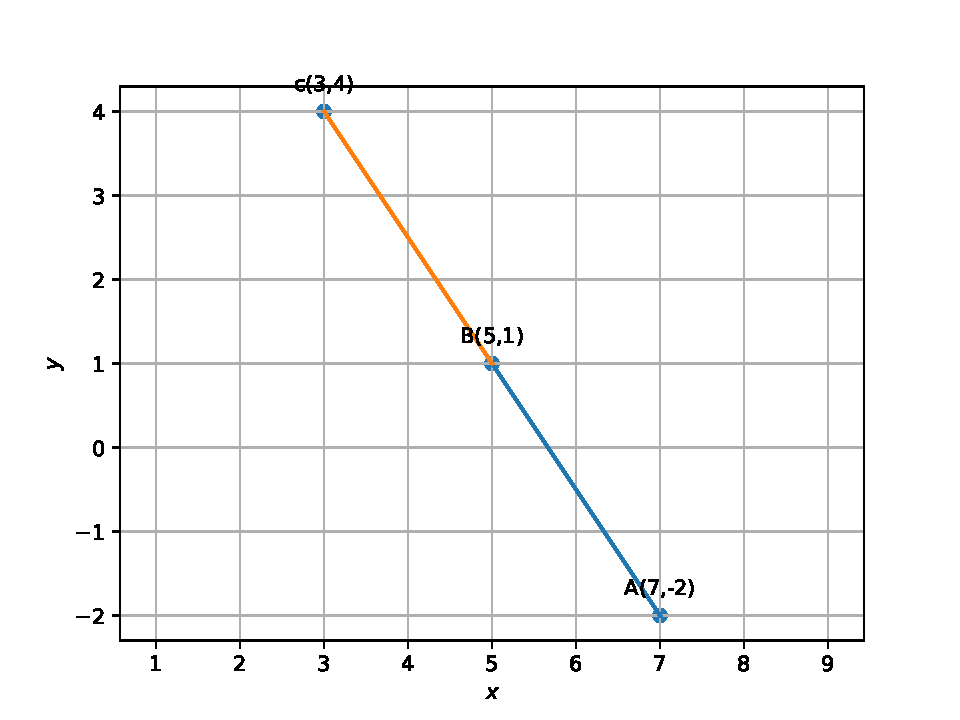
\includegraphics[width=\columnwidth]{line1.pdf}
	\end{center}
\caption{}
\label{fig:Fig1}
\end{figure}

\end{enumerate}

\end{document}
Footer
